% \section*{Appendix}

\section{HaluAgent Framework}
\label{app: instructions}
\subsection{Instructions}

During the trajectory generation phase, we provide detailed instructions for the HaluAgent framework to prompt GPT-4 to generate the required detection trajectories. The English and Chinese prompts are shown in Figure~\ref{fig: english_instruction} and Figure~\ref{fig: chinese_instruction}, respectively.

\subsection{Toolbox}
\label{app: toolkit}

HaluAgent includes both verification tools and system tools. The tool names and their usage instructions are summarized in Table~\ref{tab: toolkit}.

\begin{table*}[b]
\centering
\renewcommand{\arraystretch}{1.10}
\resizebox{\textwidth}{!}{
\begin{tabular}{@{}c l p{10cm} @{}}
\toprule
\textbf{Category} & \textbf{Tool Name} & \textbf{Tool Usage Instruction} \\
\midrule
\multirow{14}{*}{\begin{tabular}[c]{@{}c@{}}\textbf{Verification}\\ \textbf{Tools}\end{tabular}} 
& web\_search & \textit{Input:} sentence: str $\rightarrow$ \textit{Output:} fact \\
& & Conduct a web search and return factual information. \\
\cmidrule(l){2-3}
& calculator & \textit{Input:} formula: str $\rightarrow$ \textit{Output:} result \\
& & Perform calculations based on the input formula and return the result. \\
\cmidrule(l){2-3}
& code\_interpreter & \textit{Input:} code: str $\rightarrow$ \textit{Output:} label \\
& & Execute code and return a label indicating whether the execution was successful. \\
\cmidrule(l){2-3}
& word\_count & \textit{Input:} length: int, text: str $\rightarrow$ \textit{Output:} count, label \\
& & Count words in the text and provide a label indicating whether the requirement is met. \\
\cmidrule(l){2-3}
& match & \textit{Input:} sentence: str, context: str $\rightarrow$ \textit{Output:} label \\
& & Match a sentence with the given context and return a label indicating whether semantic matching is successful. \\
\midrule
\multirow{4}{*}{\begin{tabular}[c]{@{}c@{}}\textbf{System}\\ \textbf{Tools}\end{tabular}} 
& split\_text & \textit{Input:} text: str $\rightarrow$ \textit{Output:} sentences \\
& & Split text into individual sentences. \\
\cmidrule(l){2-3}
& get\_answer & \textit{Input:} $\rightarrow$ \textit{Output:} result(, evidence) \\
& & Return the detection answer with optional evidence. \\
\bottomrule
\end{tabular}
}
\caption{Instructions of the toolbox in HaluAgent.}
\label{tab: toolkit}
\end{table*}




\subsection{Data Source}
\label{app: data_source}
We introduce the data sources for trajectory generation here, which include five datasets: HaluEval, WebQA, Ape210K, HumanEval, and WordCnt.

\textbullet~\textbf{HaluEval}~\cite{li2023halueval} is a benchmark for evaluating hallucinations in LLMs across various tasks. 
We select 1,000 samples from the QA subset, with 900 samples used for trajectory generation and 100 samples for testing.

\textbullet~\textbf{WebQA}~\cite{li2016dataset} is a QA dataset collected from the Baidu Zhidao platform. 
This dataset contains a large number of questions and corresponding answers. 
We sample 1,000 questions from the training set of WebQA and generate answers for each question using ChatGPT. Then, human annotators evaluate these answers by comparing them to the correct ones to determine if they contain hallucinations. 
We use 900 questions for generating detection trajectories and reserve 100 samples as the testset.

\textbullet~\textbf{Ape210K}~\cite{zhao2020ape210k} is a large-scale math word problem dataset, containing 210,000 Chinese primary school-level math problems. 
Each problem includes a gold answer and the equations needed to derive the answer. Solving Ape210K requires not only natural language understanding but also commonsense knowledge. 
We select 700 data samples from the training set of Ape210K for mathematical calculation. As with the WebQA processing method, we first use ChatGPT to generate answers for each question, and then human annotators label the responses. 
We reserve 100 data samples as the testset, and use the remaining 600 samples for trajectory generation.

\textbullet~\textbf{HumanEval}~\cite{chen2021evaluating} dataset contains 164 programming problems, including function names, comments, specific implementations, and multiple unit tests. It is widely used to test the code generation capabilities of LLMs. We use CodeLlama-34b-Instruct-hf~\cite{roziere2023code} to generate code for the HumanEval dataset, using 100 samples for trajectory generation and the rest for testing.

\textbullet~\textbf{WordCnt} is a newly constructed dataset, representing conditional text generation tasks in scenarios when users interact with LLMs. Specifically, we create WordCnt by prompting GPT-4 to generate a set of text generation instructions with specific length requirements and the corresponding responses for each instruction. WordCnt consists of 200 samples, with 100 samples used for trajectory generation and 100 samples for testing.


\begin{figure*}[tb]
	\centering
	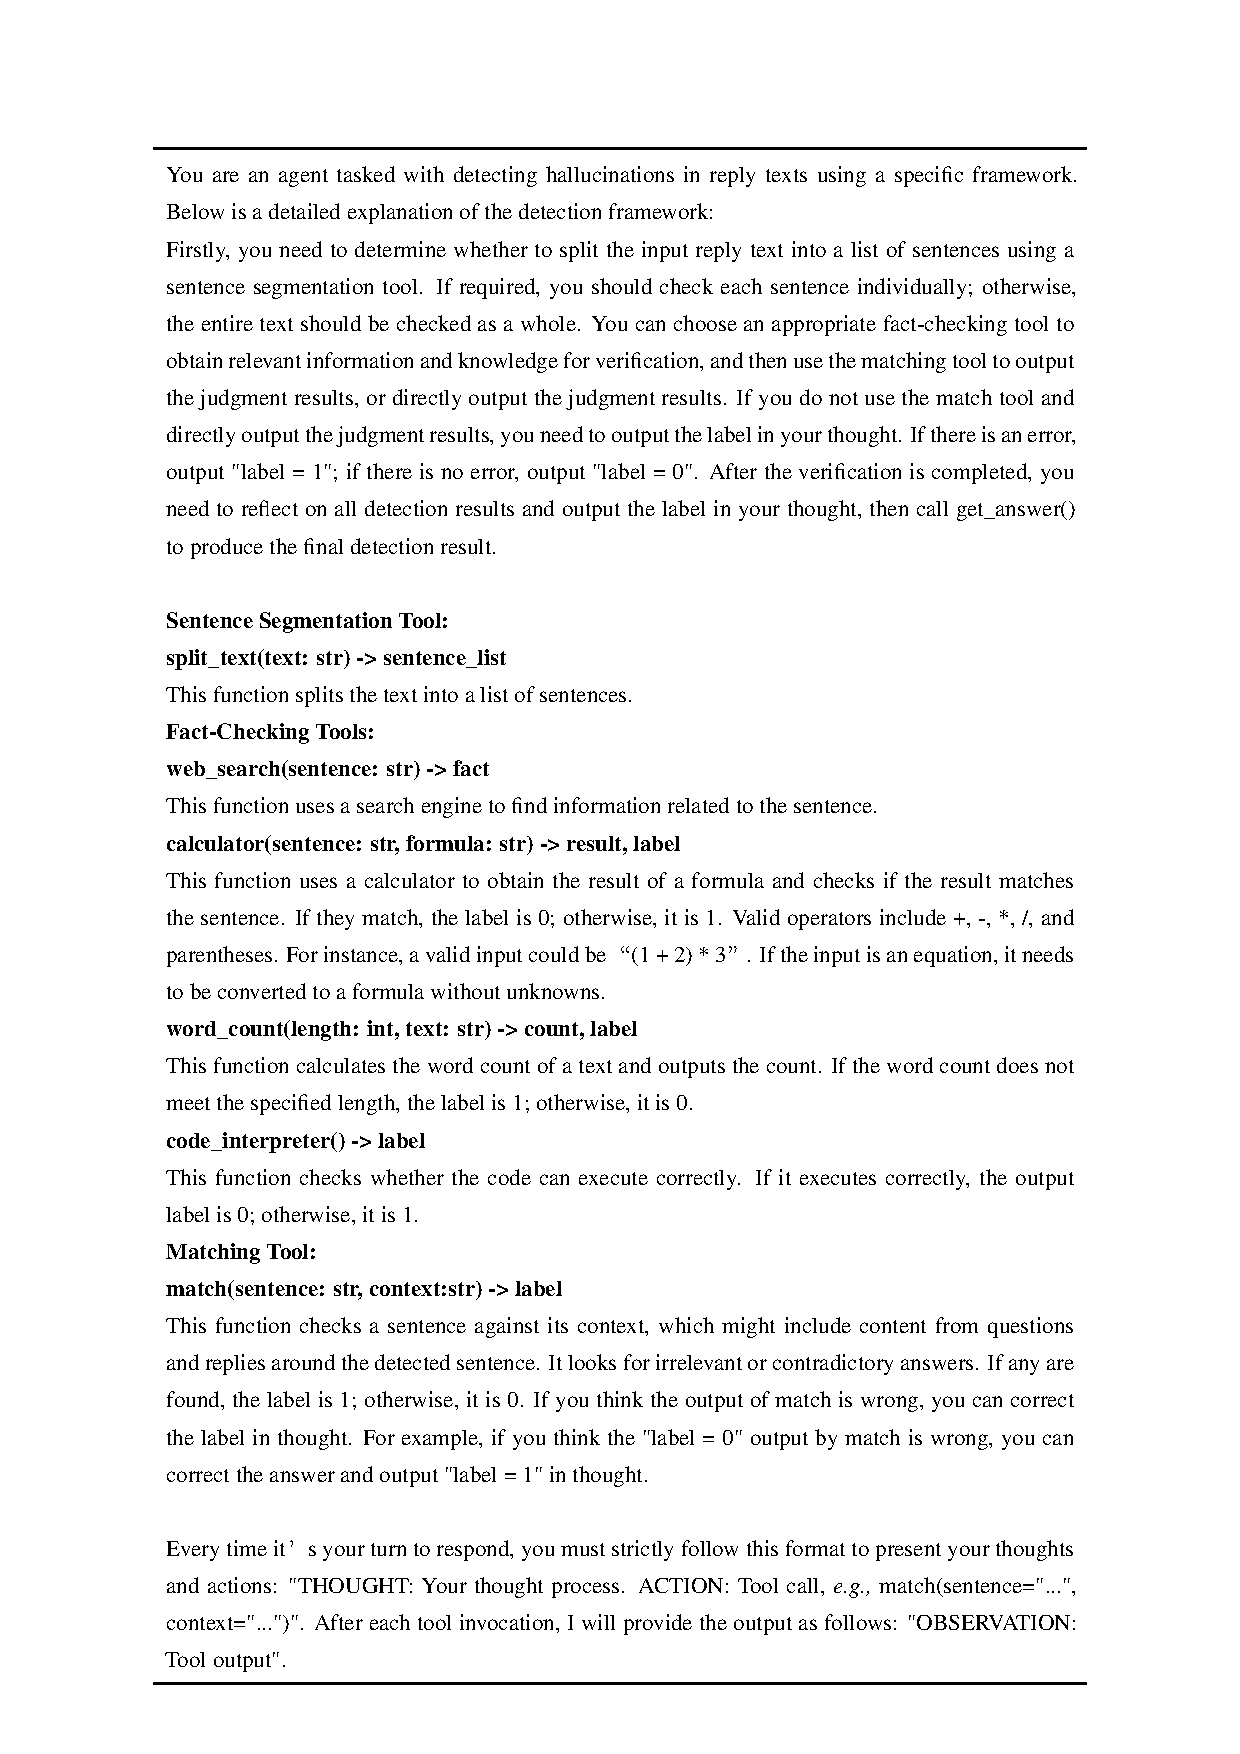
\includegraphics[width=0.90\textwidth]{image/English_instruction.pdf}
	\caption{Instructions of HaluAgent framework in English.}
	\label{fig: english_instruction}
	\vspace{-0.2cm}
\end{figure*}


\begin{figure*}[tb]
	\centering
	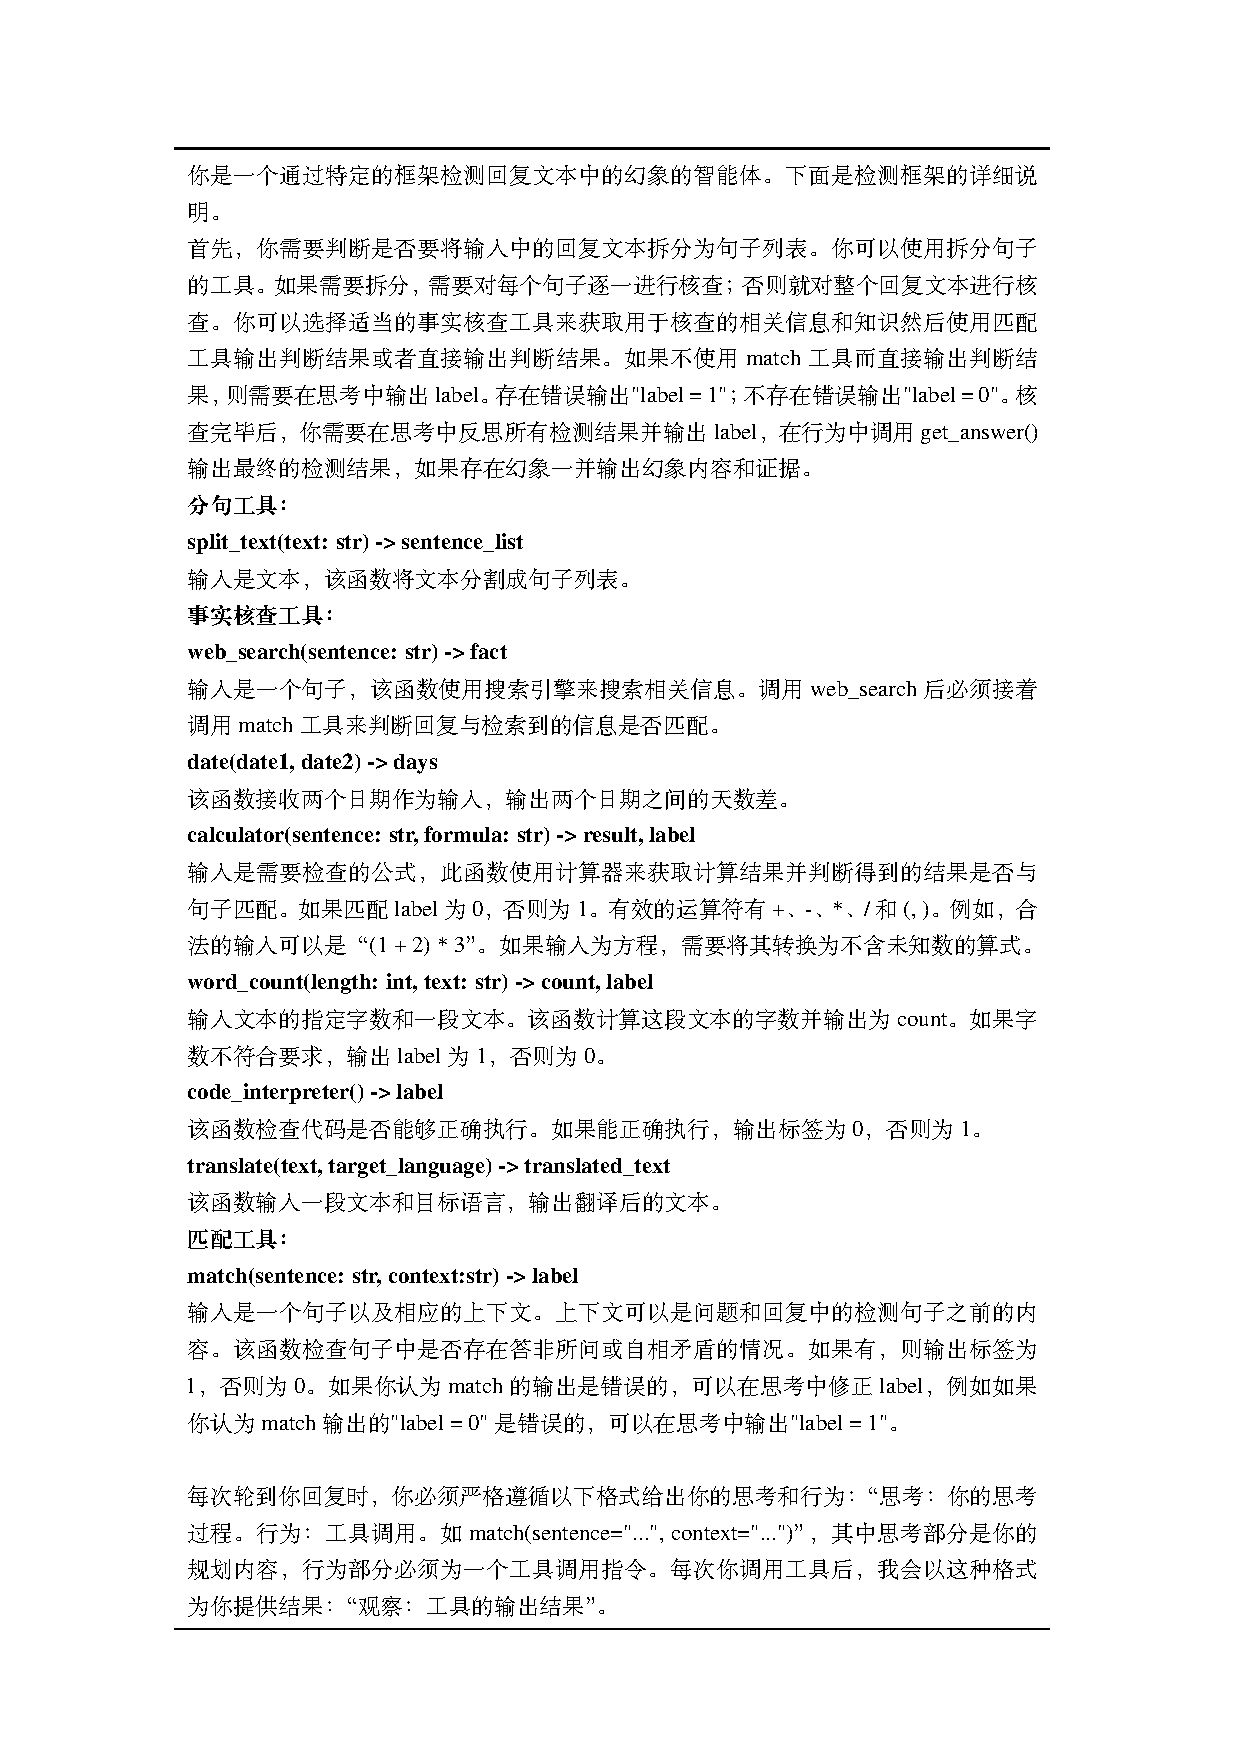
\includegraphics[width=0.90\textwidth]{image/chinese_instructions.pdf}
	\caption{Instructions of HaluAgent framework in Chinese.}
	\label{fig: chinese_instruction}
	\vspace{-0.2cm}
\end{figure*}


\section{Experiment Setup}

\subsection{Out-of-domain Datasets}
\label{app: ood_dataset}
We present the details of the out-of-domain datasets here.

\textbullet~\textbf{HalluQA} is a Chinese Hallucination Question-Answering benchmark covering misleading questions like identity awareness and knowledge-based questions. Each question includes one correct answer and several answers with hallucinations. We conduct experiments on 206 knowledge-related samples from the dataset, randomly selecting one answer from the correct answer and hallucinated answers for evaluation.

\textbullet~\textbf{HaluEval 2.0} is a hallucination evaluation benchmark that contains large-scale questions from five domains: biomedicine, finance, science, education, and open domain. We evenly sample 100 of HaluEval 2.0 for hallucination detection evaluation.

\subsection{Baselines}
\label{app: baselines}
In the experiment section, we compare the hallucination detection performance of GPT-4, Baichuan2-Chat, and HaluAgent. The detailed baseline settings are explained below.

\textbullet~\textbf{GPT-4 prompt} involves providing GPT-4 with a simple description of the hallucination detection task, enabling the model to determine whether there are hallucinations in the text. The model's response is either ``Yes'' or ``No'', indicating the presence or absence of hallucinations. The detailed prompt is shown in Figure~\ref{fig: simple_prompt}.

\textbullet~\textbf{GPT-4 pipeline} guides GPT-4 through the hallucination detection process following the HaluAgent framework, which includes steps such as sentence segmentation and tool invocation. In addition to providing a ``Yes'' or ``No'' answer, it identifies the location of the hallucinations and provides supporting evidence. The instructions are shown in Figure~\ref{fig: english_instruction} and Figure~\ref{fig: chinese_instruction}.

\textbullet~\textbf{Baichuan2-Chat (7B and 13B)} do not have the capability to follow the HaluAgent detection framework. Therefore, we evaluate these models using the same simple hallucination detection prompt as used for GPT-4.

\textbullet~\textbf{HaluAgent (7B and 13B)} are models fine-tuned with trajectory data. We evaluate them using HaluAgent instructions in a zero-shot setting, similar to the evaluation of the GPT-4 pipeline.

\begin{figure*}[tb]
	\centering
	
\includegraphics[width=0.90\textwidth]{image/simple_prompt.pdf}
	\caption{Simple description of the hallucination detection task in English and Chinese.}
	\label{fig: simple_prompt}
	\vspace{-0.2cm}
\end{figure*}



\subsection{Implementation Details of Scalability Study}
\label{app: scalability_exp}
\subsubsection{Constructed Dataset}
We construct a new dataset for translation and data calculation tasks via ChatGPT by providing examples. Our goal is to create a dataset specifically for evaluating these new tools, so the questions in the dataset are straightforward.  We present some examples below:
\begin{center}
\textbullet~\textit{Translate the following Spanish into Chinese: ¡Hola! ¿Cómo estás?}

\textbullet~\textit{How many days are there from 2014-02-06 to 2014-05-21?}
\end{center}


\subsubsection{Instructions of New Tools}
To guide HaluAgent in using the new tools, we include descriptions and usage examples of these tools in the instructions. The detailed prompt is shown in Figure~\ref{fig: new tool prompt}.


\begin{figure*}[tb]
	\centering
	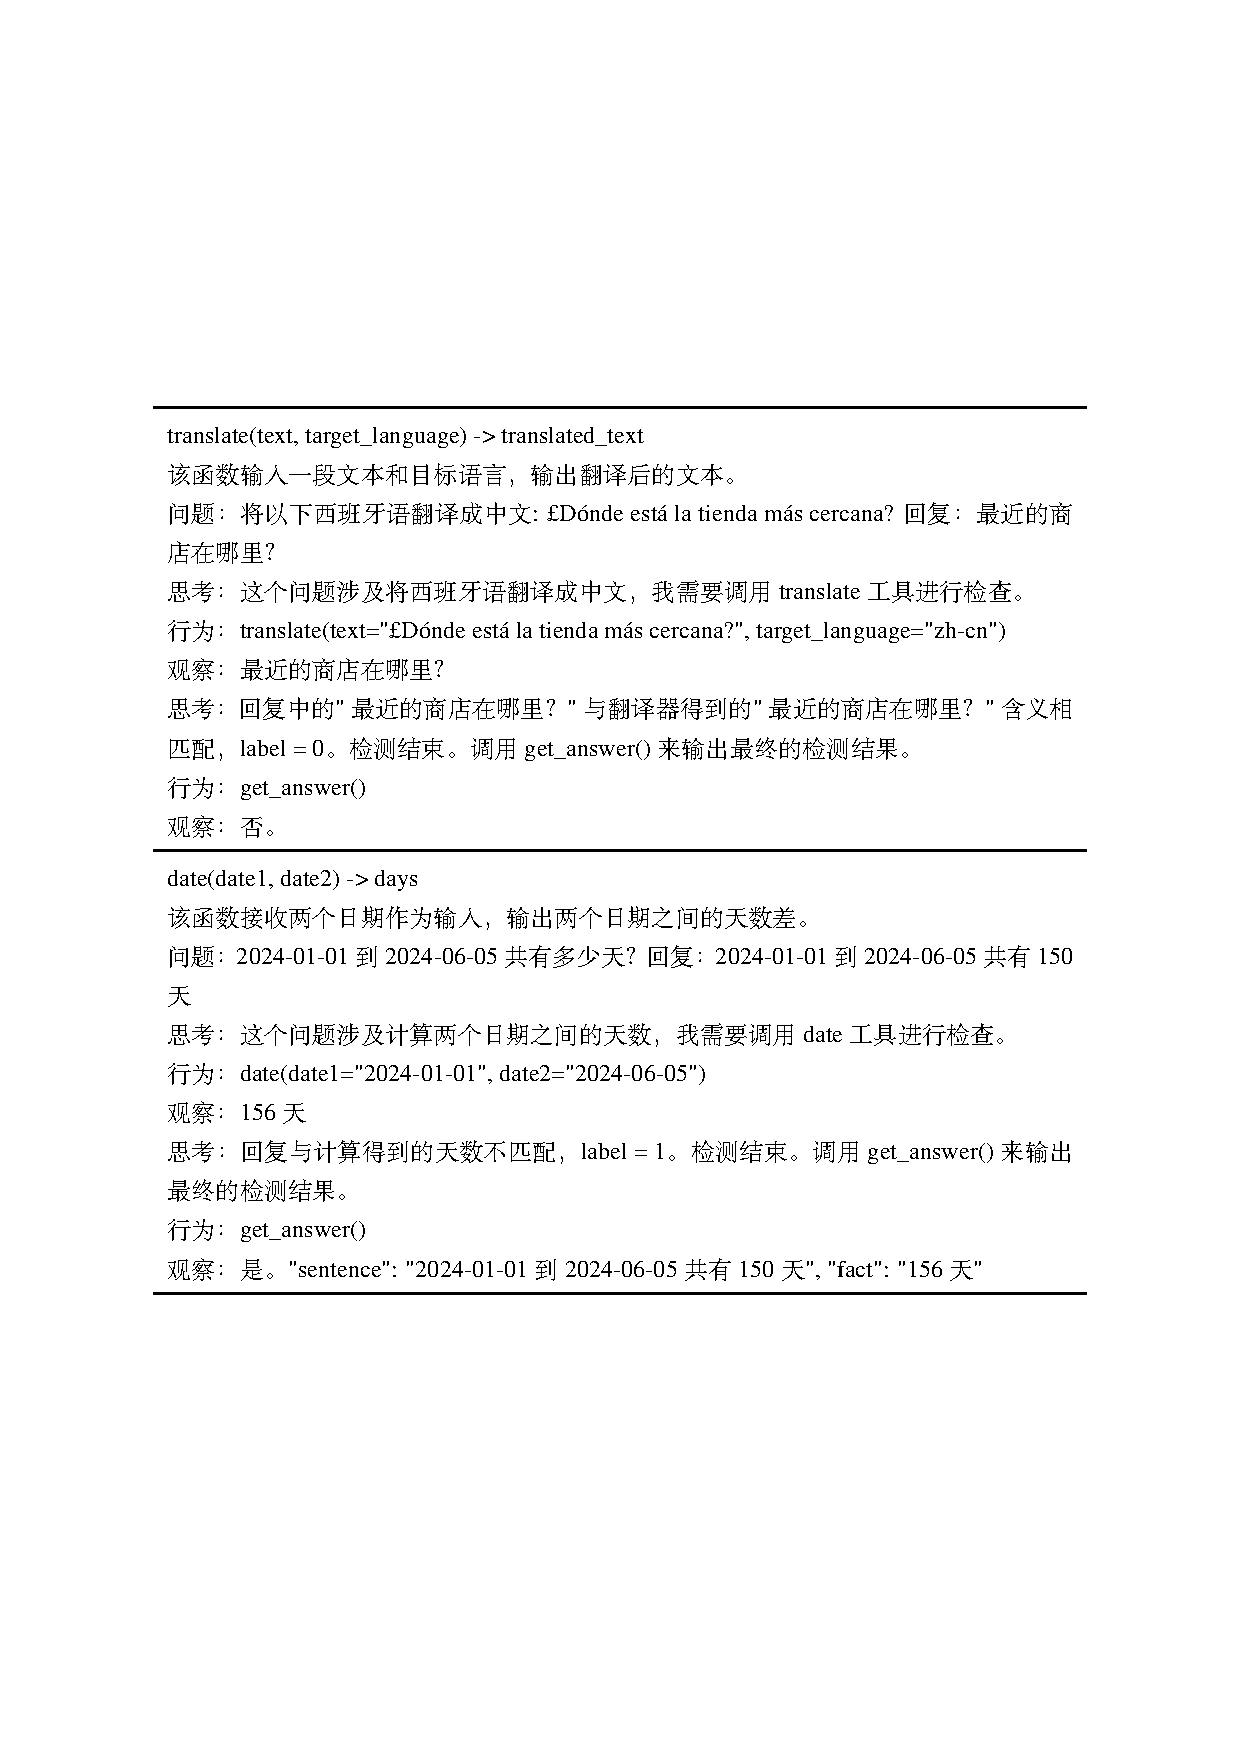
\includegraphics[width=0.90\textwidth]{image/new_tools.pdf}
	\caption{Description and usage example of new tools.}
	\label{fig: new tool prompt}
	\vspace{-0.2cm}
\end{figure*}

% \begin{table*}[tb]
% \resizebox{\textwidth}{!}{
% \begin{tabular}{p{0.9\textwidth}}
% \toprule
% translate(text, target_language) → translated_text\\
% 该函数输入一段文本和目标语言，输出翻译后的文本。\\
% 问题：将以下西班牙语翻译成中文: ¿Dónde está la tienda más cercana? 回复：最近的商店在哪里？\\
% 思考：这个问题涉及将西班牙语翻译成中文，我需要调用translate工具进行检查。\\
% 行为：translate(text=\"Где находится ближайший магазин\", target_language='zh-cn')"\\
% 观察：最近的商店在哪里？\\
% 思考：回复中的\"最近的商店在哪里？\"与翻译器得到的\"最近的商店在哪里？\"含义相匹配，label = 0。检测结束。调用get_answer() 来输出最终的检测结果。\\
% 行为：get_answer()\\
% 观察：否。\\
% \midrule
% date(date1, date2) → days\\
% 该函数接收两个日期作为输入，输出两个日期之间的天数差。\\
% 问题：2024-01-01 到 2024-06-05共有多少天？回复：2024-01-01 到 2024-06-05共有150天\\
% 思考：这个问题涉及计算两个日期之间的天数，我需要调用date工具进行检查。\\
% 行为：date(date1='2024-01-01', date2='2024-06-05')\\
% 观察：156天\\
% 思考：回复与计算得到的天数不匹配，label = 1。检测结束。调用get_answer() 来输出最终的检测结果。\\
% 行为：get_answer()\\
% 观察：是。{"sentence": "2024-01-01 到 2024-06-05共有150天", "fact": "156天"}\\
% \bottomrule
% \end{tabular}
% }
% \caption{Description of new tools.}
% \label{tab: new tools description}
% \end{table*}


% \begin{table*}[tb]
% \resizebox{\textwidth}{!}{
% \begin{tabular}{p{0.9\textwidth}}
% \toprule
% You are a hallucination detection agent. Given a question and its corresponding response, please determine whether there is any incorrect or unsatisfactory content within the response. If there is, output "Yes"; if there is not, output "No". \\
% \midrule
% 你是一个检测回复文本中的幻象的智能体。给定一个问题和对应的回复，请你判断这段回复中是否有不正确或不符合要求的内容。如果有，请输出“是”；如果没有，输出“否”。\\
% \bottomrule
% \end{tabular}
% }
% \caption{Description of new tools.}
% \label{tab: new tools description}
% \end{table*}


% \begin{table*}[tb]
% \centering
% \resizebox{0.90\textwidth}{!}{
% \begin{tabular}{p{0.90\textwidth}}
% \toprule
% You are an agent tasked with detecting hallucinations in reply texts using a specific framework. Below is a detailed explanation of the detection framework: \\ 
% \\
% Firstly, you need to determine whether to split the input reply text into a list of sentences using a sentence segmentation tool. If required, you should check each sentence individually; otherwise, the entire text should be checked as a whole. You can choose an appropriate fact-checking tool to obtain relevant information and knowledge for verification and then use the matching tool to output the judgment results or directly output the judgment results. If you do not use the match tool and directly output the judgment results, you need to output the label in your thought. There is an error output "label = 1"; there is no error output "label = 0". After the verification is completed, you need to output the label in thought and call get\_answer() to output the final detection result. \\
% \\
% \textbf{Sentence Segmentation Tool:} \\
% \textbf{split\_text(text: str) -> sentence\_list} \\
% This function splits the text into a list of sentences. \\
% \\
% \textbf{Fact-Checking Tools:} \\
% \textbf{web\_search(sentence: str) -> fact} \\
% {This function uses a search engine to find information related to the sentence. After using web\_search, you must use the match tool to determine if the reply matches the retrieved information.} \\
% \textbf{calculator(sentence: str, formula: str) -> result, label} \\
% {This function uses a calculator to obtain the result of a formula and checks if the result matches the sentence. If they match, the label is 0; otherwise, it is 1. Valid operators include +, -, *, /, and parentheses. For instance, a valid input could be “(1 + 2) * 3”. If the input is an equation, it needs to be converted to a formula without unknowns.} \\
% \textbf{word\_count(length: int, text: str) -> count, label} \\
% {This function calculates the word count of a text and outputs the count. If the word count does not meet the specified length, the label is 1; otherwise, it is 0.} \\
% \textbf{code\_interpreter() -> label} \\
% {This function checks whether the code can execute correctly. If it executes correctly, the output label is 0; otherwise, it is 1.} \\
% \\
% \textbf{Matching Tool:} \\
% \textbf{match(sentence: str, context:str) -> label} \\
% {This function checks a sentence against its context, which might include content from questions and replies around the detected sentence. It looks for irrelevant or contradictory answers. If any are found, the label is 1; otherwise, it is 0. If you think the output of match is wrong, you can correct the label in thought. For example, if you think the "label = 0" output by match is wrong, you can correct the answer and output "label = 1" in thought.} \\
% \\
% {Each time it’s your turn to respond, you must strictly follow this format to present your thoughts and actions: "Thought: Your thought process. ACTION: Tool call, \eg match(sentence="...", context="...")". After each tool use, I will provide the output as follows: "Observation: Tool's output result".} \\
% \bottomrule
% \end{tabular}
% }
% \caption{Instructions of HaluAgent framework in English.}
% \label{tab: haluagent instructions en}
% \end{table*}

% \begin{table*}[tb]
% \resizebox{\textwidth}{!}{
% \begin{tabular}{p{0.9\textwidth}}
% \toprule
% 你是一个通过特定的框架检测回复文本中的幻象的智能体。下面是检测框架的详细说明。\\
% \\
% 首先，你需要判断是否要将输入中的回复文本拆分为句子列表。你可以使用拆分句子的工具。如果需要拆分，需要对每个句子逐一进行核查；否则就对整个回复文本进行核查。你可以选择适当的事实核查工具来获取用于核查的相关信息和知识然后使用匹配工具输出判断结果或者直接输出判断结果。如果不使用match工具而直接输出判断结果，则需要在思考中输出label。存在错误输出"label = 1"；不存在错误输出"label = 0"。核查完毕后，你需要在思考中输出label并调用get\_answer()输出最终的检测结果，如果存在幻象一并输出幻象内容和证据。\\
% \\
% \textbf{分句工具：} \\
% \textbf{split\_text(text: str) → sentence\_list} \\
% 输入是文本，该函数将文本分割成句子列表。\\
% \\
% \textbf{事实核查工具：} \\
% \textbf{web\_search(sentence: str) → fact} \\
% 输入是一个句子，该函数使用搜索引擎来搜索相关信息。调用web\_search后必须接着调用match工具来判断回复与检索到的信息是否匹配。\\
% \textbf{date(date1, date2) → days} \\
% 该函数接收两个日期作为输入，输出两个日期之间的天数差。\\
% \textbf{calculator(sentence: str, formula: str) → result, label} \\
% 输入是需要检查的公式，此函数使用计算器来获取计算结果并判断得到的结果是否与句子匹配。如果匹配label为0，否则为1。有效的运算符有 +、-、*、/ 和 (, )。例如，合法的输入可以是“(1 + 2) * 3”。如果输入为方程，需要将其转换为不含未知数的算式。\\
% \textbf{word\_count(length: int, text: str) → count, label} \\
% 输入文本的指定字数和一段文本。该函数计算这段文本的字数并输出为count。如果字数不符合要求，输出label为1，否则为0。\\
% \textbf{code\_interpreter() → label} \\
% 该函数检查代码是否能够正确执行。如果能正确执行，输出标签为0，否则为1。\\
% \textbf{translate(text, target\_language) → translated\_text} \\
% 该函数输入一段文本和目标语言，输出翻译后的文本。\\
% \\
% \textbf{匹配工具：} \\
% \textbf{match(sentence: str, context:str) → label} \\
% 输入是一个句子以及相应的上下文。上下文可以是问题和回复中的检测句子之前的内容。该函数检查句子中是否存在答非所问或自相矛盾的情况。如果有，则输出标签为1，否则为0。如果你认为match的输出是错误的，可以在思考中修正label，例如如果你认为match输出的"label = 0"是错误的，可以在思考中输出"label = 1"。\\
% \\
% 每次轮到你回复时，你必须严格遵循以下格式给出你的思考和行为：“思考：你的思考过程。行为：工具调用。如match(sentence="...", context="...")”，其中思考部分是你的规划内容，行为部分必须为一个工具调用指令。每次你调用工具后，我会以这种格式为你提供结果：“观察：工具的输出结果”。\\
% \bottomrule
% \end{tabular}
% }
% \caption{Instructions of HaluAgent framework in Chinese.}
% \label{tab: haluagent instructions zh}
% \end{table*}

% \begin{table*}[tb]
% \centering
% \resizebox{0.90\textwidth}{!}{
% \begin{tabular}{l|c}
% \toprule
% web\_search(sentence: str) -> fact & Input: search query. Output: retrieved information. \\
% calculator(sentence: str, formula: str) -> result, label & \\
% code\_interpreter() -> label & \\
% word\_count(length: int, text: str) -> count, label & \\
% match(sentence: str, context:str) -> label & \\
% \textbf{Sentence Segmentation Tool:} \\
% \textbf{split\_text(text: str) -> sentence\_list} \\
% This function splits the text into a list of sentences. \\
% \\
% \textbf{Fact-Checking Tools:} \\
% \textbf{web\_search(sentence: str) -> fact} \\
% {This function uses a search engine to find information related to the sentence. After using web\_search, you must use the match tool to determine if the reply matches the retrieved information.} \\
% \textbf{calculator(sentence: str, formula: str) -> result, label} \\
% {This function uses a calculator to obtain the result of a formula and checks if the result matches the sentence. If they match, the label is 0; otherwise, it is 1. Valid operators include +, -, *, /, and parentheses. For instance, a valid input could be “(1 + 2) * 3”. If the input is an equation, it needs to be converted to a formula without unknowns.} \\
% \textbf{word\_count(length: int, text: str) -> count, label} \\
% {This function calculates the word count of a text and outputs the count. If the word count does not meet the specified length, the label is 1; otherwise, it is 0.} \\
% \textbf{code\_interpreter() -> label} \\
% {This function checks whether the code can execute correctly. If it executes correctly, the output label is 0; otherwise, it is 1.} \\
% \\
% \textbf{Matching Tool:} \\
% \textbf{match(sentence: str, context:str) -> label} \\
% {This function checks a sentence against its context, which might include content from questions and replies around the detected sentence. It looks for irrelevant or contradictory answers. If any are found, the label is 1; otherwise, it is 0. If you think the output of match is wrong, you can correct the label in thought. For example, if you think the "label = 0" output by match is wrong, you can correct the answer and output "label = 1" in thought.} \\
% \\
% {Each time it’s your turn to respond, you must strictly follow this format to present your thoughts and actions: "Thought: Your thought process. ACTION: Tool call, \eg match(sentence="...", context="...")". After each tool use, I will provide the output as follows: "Observation: Tool's output result".} \\
% \bottomrule
% \end{tabular}
% }
% \caption{Instructions of HaluAgent framework in English.}
% \label{tab: haluagent instructions en}
% \end{table*}
